% Shared preamble for the meander paper series (papers A-D). Compile each paper with tectonic.
\usepackage[T1]{fontenc}
\usepackage[margin=1.15in]{geometry}
\usepackage{amsmath,amssymb,amsthm}
\usepackage{booktabs,array}
\usepackage{float}
\usepackage{tikz}
\usetikzlibrary{arrows.meta,decorations.pathmorphing,positioning}
\usepackage{pgfplots}
\pgfplotsset{compat=1.16}
\usepackage[colorlinks=true,linkcolor=blue!50!black,citecolor=blue!50!black,urlcolor=blue!50!black]{hyperref}

\newtheorem{theorem}{Theorem}
\newtheorem{proposition}[theorem]{Proposition}
\newtheorem{lemma}[theorem]{Lemma}
\newtheorem{corollary}[theorem]{Corollary}
\newtheorem{conjecture}[theorem]{Conjecture}
\theoremstyle{definition}
\newtheorem{definition}[theorem]{Definition}
\theoremstyle{remark}
\newtheorem*{remark}{Remark}

\emergencystretch=2em
\raggedbottom

% Tapes of the tape machine. Write -{}- for a double minus inside \tape{...} to avoid the
% typewriter dash ligature.
\newcommand{\tape}[1]{\texttt{#1}}
\newcommand{\hd}[1]{\texttt{[#1]}}

% Series line under the title.
\newcommand{\seriesline}[1]{\par\smallskip{\small\itshape Meander numbers: growth rate and exponent. #1}}

% The running example (order 3): upper arches (1,2), (3,6), (4,5); lower arches (1,6), (2,5), (3,4).
\newcommand{\meanderroad}{%
  \draw (1,0) arc[start angle=180,end angle=0,radius=0.5];
  \draw (3,0) arc[start angle=180,end angle=0,radius=1.5];
  \draw (4,0) arc[start angle=180,end angle=0,radius=0.5];
  \draw (1,0) arc[start angle=180,end angle=360,radius=2.5];
  \draw (2,0) arc[start angle=180,end angle=360,radius=1.5];
  \draw (3,0) arc[start angle=180,end angle=360,radius=0.5];
}
\newcommand{\meanderfigure}{%
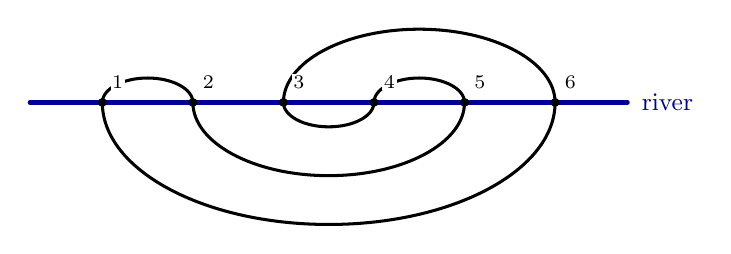
\begin{tikzpicture}[x=1.15cm,y=0.62cm,line cap=round]
  \draw[blue!60!black,line width=1.6pt] (0.2,0)--(6.8,0);
  \node[blue!60!black,anchor=west] at (6.85,0) {\small river};
  \begin{scope}[line width=1.1pt]\meanderroad\end{scope}
  \foreach \k in {1,...,6} {\fill (\k,0) circle[radius=1.6pt]; \node[fill=white,inner sep=0.6pt,font=\scriptsize] at (\k+0.17,0.42) {\k};}
\end{tikzpicture}}

% The series. Each paper cites the others as \cite{PaperA} etc.
